\documentclass{beamer}
\usetheme{default}
\beamertemplatenavigationsymbolsempty
\usepackage{rembeamer}

\begin{document}

\begin{frame}
  \begin{itemize}
    \item[] 
      LO13: Using the normal distribution to find z-scores and
      percentiles.
  \end{itemize}
\end{frame}

\begin{frame}
  \frametitle{Distribution}
  \centering
  \begin{tikzpicture}
    \begin{axis}[
      xmin=5,
      xmax=25,
      xlabel={Interest Rate (Percentage)},
      ylabel={Count}
    ]
      \addplot+ [
        hist={bins=8},
        fill=orange,
        draw=black,
        mark=none
      ]
      table [y=interest_rate,col sep=tab] {../data/loans50.dat};
    \end{axis}
  \end{tikzpicture}
\end{frame}

\begin{frame}
  \frametitle{Normal Distribution}
  \centering
  \begin{tikzpicture}
    \begin{axis}[
      xlabel={Population},
      ylabel={Count}
      ]
      \addplot+ [
        hist={bins=9},
        fill=orange,
        draw=black,
        mark=none
      ]
      table [y=count,col sep=comma] {../data/normal.dat};
    \end{axis}
  \end{tikzpicture}
\end{frame}

\begin{frame}
  \frametitle{Normal Distribution}
  \centering
  \begin{tikzpicture}
    \begin{axis}[
        ytick=\empty,
        xlabel=$\frac{1}{\sqrt{8\pi}} e^{\frac{-x^2}{8}}$,
      ]
      \addplot [
        domain=-6:6,
        samples=201,
      ]
      {exp(-x^2 / (2*2^2)) / (sqrt(2*pi*2^2))};
    \end{axis}
  \end{tikzpicture}
\end{frame}

\begin{frame}
  \frametitle{Normal Distribution}
  \begin{displaymath}
    \begin{array}{rcl}
      \mu & = & \text{Mean} \\[2em]
      \sigma & = & \text{Standard Deviation}\\[2em]
      f(x) & = & \frac{1}{\sqrt{2\pi \sigma^2}}
      e^{\frac{-(x-\mu)^2}{2\sigma^2}}
    \end{array}
  \end{displaymath} 
\end{frame}

\begin{frame}
  \frametitle{Normal Distribution}
  \centering
  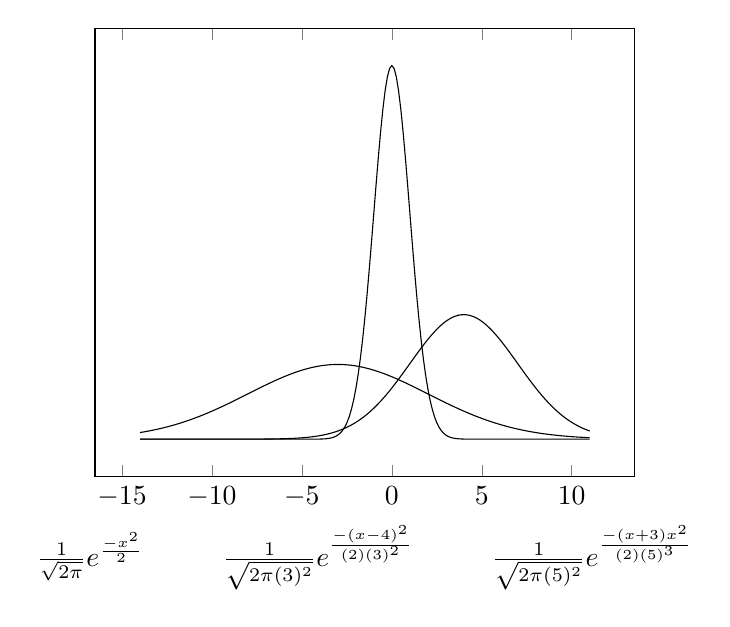
\begin{tikzpicture}
    \begin{axis}[
        ytick=\empty,
        xlabel=$
        \frac{1}{\sqrt{2\pi}} e^{\frac{-x^2}{2}} \hspace{1cm}
        \frac{1}{\sqrt{2\pi (3)^2}} e^{\frac{-(x-4)^2}{(2)(3)^2}}
        \hspace{1cm}
        \frac{1}{\sqrt{2\pi (5)^2}} e^{\frac{-(x+3)x^2}{(2)(5)^3}}
        $,
      ]
      \addplot [
        domain=-14:11,
        samples=201,
      ]
      {exp(-(x-4)^2 / (2*3^2)) / (sqrt(2*pi*3^2))};
      \addplot [
        domain=-14:11,
        samples=201,
      ]
      {exp(-x^2 / 2) / (sqrt(2*pi))};
      \addplot [
        domain=-14:11,
        samples=201,
      ]
      {exp(-(x+3)^2 / (2*5^2)) / (sqrt(2*pi*5^2))};
    \end{axis}
  \end{tikzpicture}
\end{frame}

\begin{frame}
  \frametitle{z-Scores}
  \begin{displaymath}
    \begin{array}{rcl}
      \mu & = & \text{Mean} \\[2em]
      \sigma & = & \text{Standard Deviation}\\[2em]
      f(x) & = & \frac{1}{\sqrt{2\pi \sigma^2}}
      e^{\frac{-(x-\mu)^2}{2\sigma^2}} \\[2em]
      z(x) & = & \frac{x-\mu}{\sigma} 
    \end{array}
  \end{displaymath} 
\end{frame}

\begin{frame}
  \frametitle{Normal Distribution and z-Scores}
  \centering
  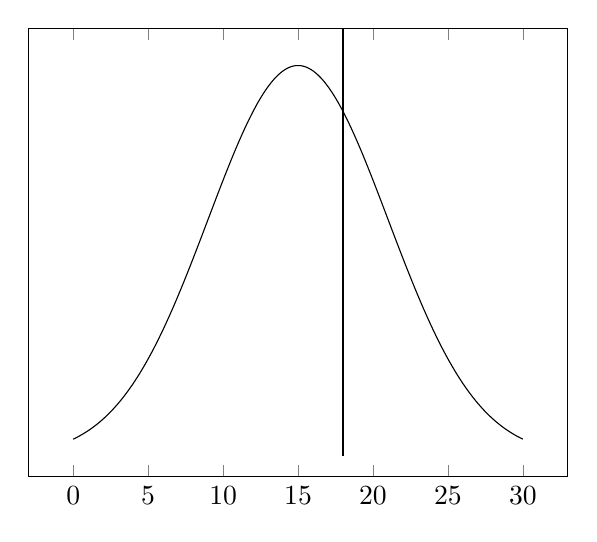
\begin{tikzpicture}
    \begin{axis}[
        ytick=\empty,
      ]
      \addplot [
        domain=0:30,
        samples=201,
      ]
      {exp(-(x-15)^2 / (2*(6)^2)) / (sqrt(2*pi*(6)^2))};
      \draw (18,0) -- (18,0.4);
    \end{axis}
  \end{tikzpicture}
  \begin{equation*}
    \mu = 15 \quad \sigma = 6 \quad z(18) = \frac{18-15}{6} =
    \frac{3}{6} = 0.5
  \end{equation*}
\end{frame}

\begin{frame}
  \frametitle{z-Scores and Percentiles}
  \centering
  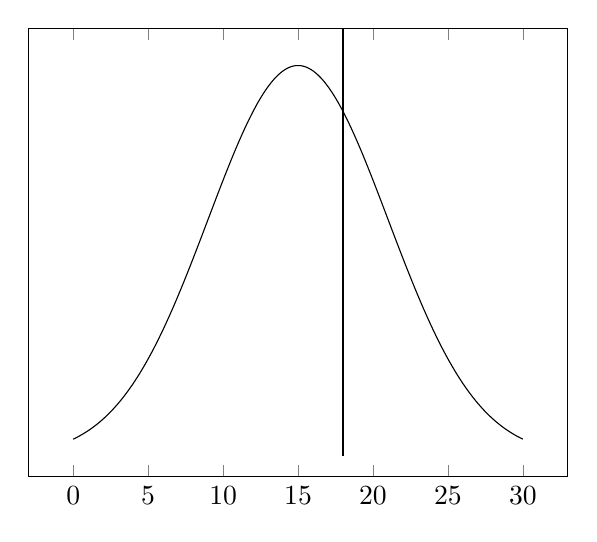
\begin{tikzpicture}
    \begin{axis}[
        ytick=\empty,
      ]
      \addplot [
        domain=0:30,
        samples=201,
      ]
      {exp(-(x-15)^2 / (2*(6)^2)) / (sqrt(2*pi*(6)^2))};
      \draw (18,0) -- (18,0.4);
    \end{axis}
  \end{tikzpicture}
  \begin{equation*}
    z(18) = 0.5 \mapsto 0.691 \mapsto 69.1\% \quad 30.9\%
  \end{equation*}
\end{frame}

\begin{frame}
  \frametitle{Sample Distribution}
  \centering
  \begin{tikzpicture}
    \begin{axis}[
      xmin=5,
      xmax=25,
      xlabel={Interest Rate (Percentage)},
      ylabel={Count}
    ]
      \addplot+ [
        hist={bins=8},
        fill=orange,
        draw=black,
        mark=none
      ]
      table [y=interest_rate,col sep=tab] {../data/loans50.dat};
    \end{axis}
  \end{tikzpicture}
\end{frame}

\begin{frame}
  \frametitle{Random Trials}
  \begin{displaymath}
    \begin{tabular}{@{}ccc@{}}
      \toprule
      men promoted & women promoted & difference \\[0.3em]
      \cmidrule(r){1-1} \cmidrule(lr){2-2} \cmidrule(lr){3-3}
      20 & 15 & 0.208 \\
      22 & 13 & 0.357 \\
      15 & 20 & -0.208 \\ 
      20 & 15 & 0.208 \\
      11 & 24 & -0.542 \\  
      19 & 16 & 0.125 \\
      20 & 15 & 0.208 \\ 
      14 & 21 & -0.292 \\
      18 & 17 & 0.042 \\  
      12 & 23 & -0.458 \\
      \bottomrule
    \end{tabular}
  \end{displaymath} 
\end{frame}

\begin{frame}
  \frametitle{Sampling Distribution}
  \centering
  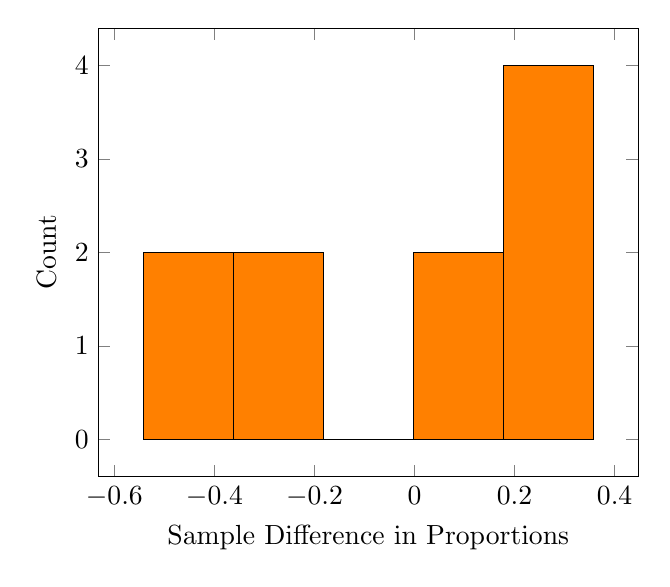
\begin{tikzpicture}
    \begin{axis}[
      xlabel={Sample Difference in Proportions},
      ylabel={Count}
    ]
      \addplot+ [
        hist={bins=5},
        fill=orange,
        draw=black,
        mark=none
      ]
      table [row sep=\\,y index=0] {
      0.208 \\
      0.357 \\
      -0.208 \\ 
      0.208 \\
      -0.542 \\  
      0.125 \\
      0.208 \\ 
      -0.292 \\
      0.042 \\  
      -0.458 \\
      };
    \end{axis}
  \end{tikzpicture}
\end{frame}

\begin{frame}
  \frametitle{Distributions}
  \begin{itemize}
    \item[] 
      Parameter: proportion or difference in proportions.
      \vspace{0.5cm}
    \item[] 
      Population Distribution
      \vspace{0.5cm}
    \item[] 
      Sample Statistic: proportion or difference in proportions.
      \vspace{0.5cm}
    \item[] 
      Sampling Distribution
  \end{itemize}
\end{frame}

\begin{frame}
  \frametitle{Central Limit Theorem}
  \begin{itemize}
    \item[] 
      The statistic is a proportion or difference in a proportion.
      \vspace{0.5cm}
    \item[] 
      The observations in the samples are independent.
      \vspace{0.5cm}
    \item[] 
      The sample is large enough. 
      \vspace{0.5cm}
    \item[] 
      Then the sampling distribution will be roughly normal, and will
      become closer and closer to normal as the sample size increases.
  \end{itemize}
\end{frame}

\end{document}


\begin{frame}
  \frametitle{p-value}
  \begin{itemize}
    \item[] 
      Many, many random trials. 
      \vspace{0.5cm}
    \item[] 
      Promotion proportion difference $\geq 0.292$ happened about
      $2\%$ of the time. $p = 0.02$. 
      \vspace{0.5cm}
    \item[] 
      $2\%$ change that $H_0$ is true and our sample statistics was
      just random variance in the population. 
      \vspace{0.5cm}
    \item[] 
      Significance level $\alpha$. 
      \vspace{0.5cm}
    \item[] 
      $p < \alpha$ is called `statistically significant'. 
      \vspace{0.5cm}
    \item[] 
      Often $\alpha = 0.05$. If so, our sample statistics is
      significant to reject $H_0$.
    \item[] 
  \end{itemize}
\end{frame}

\end{document}


